\documentclass[a4paper,titlepage]{article}

% use this when images are included
\usepackage{float}
\usepackage{graphicx}
\usepackage{subcaption}
\graphicspath{ {./images/} }

% use for lines of code
\usepackage{listings}

% use for links, also links list of contents
\usepackage{hyperref}

\title{The Varroa Destructor Destructor}
\date{2021\\ April - August}
%\author{Max-Felix Müller\\ \\ 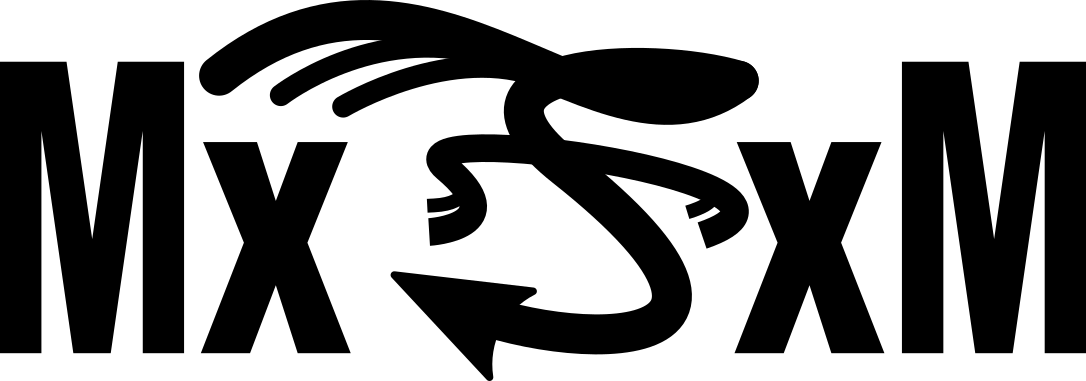
\includegraphics[width=\textwidth]{mxfxm.png}}
\author{TGMB The German Mite Busters\\ Max-Felix Müller, Adam Theo Müller, Lukas Dietz, Frank Münzer\\ \\ 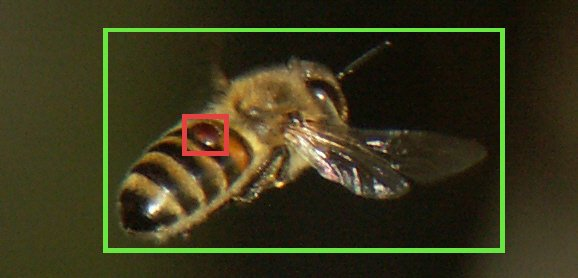
\includegraphics[width=\textwidth]{Biene_mit_Varroa_erkannt.jpg}}

\begin{document}
\maketitle
\tableofcontents
\newpage
\listoffigures %delete if not necessary
\listoftables %delete if not necessary
\newpage

\section*{Abstract}

\newpage
\section{OpenCV AI Competition 2021}

\href{https://opencv.org/opencv-ai-competition-2021/}{https://opencv.org/opencv-ai-competition-2021/} \\

The OpenCV AI Competition focuses on solving real world problems using spatial AI and the OAK-D camera.
The event is sponsored by Microsoft Azure and Intel.

\subsection{Regions}

Different parts of the world have different problems to solve, so the map was split into 6 regions.

\begin{figure}[H]
    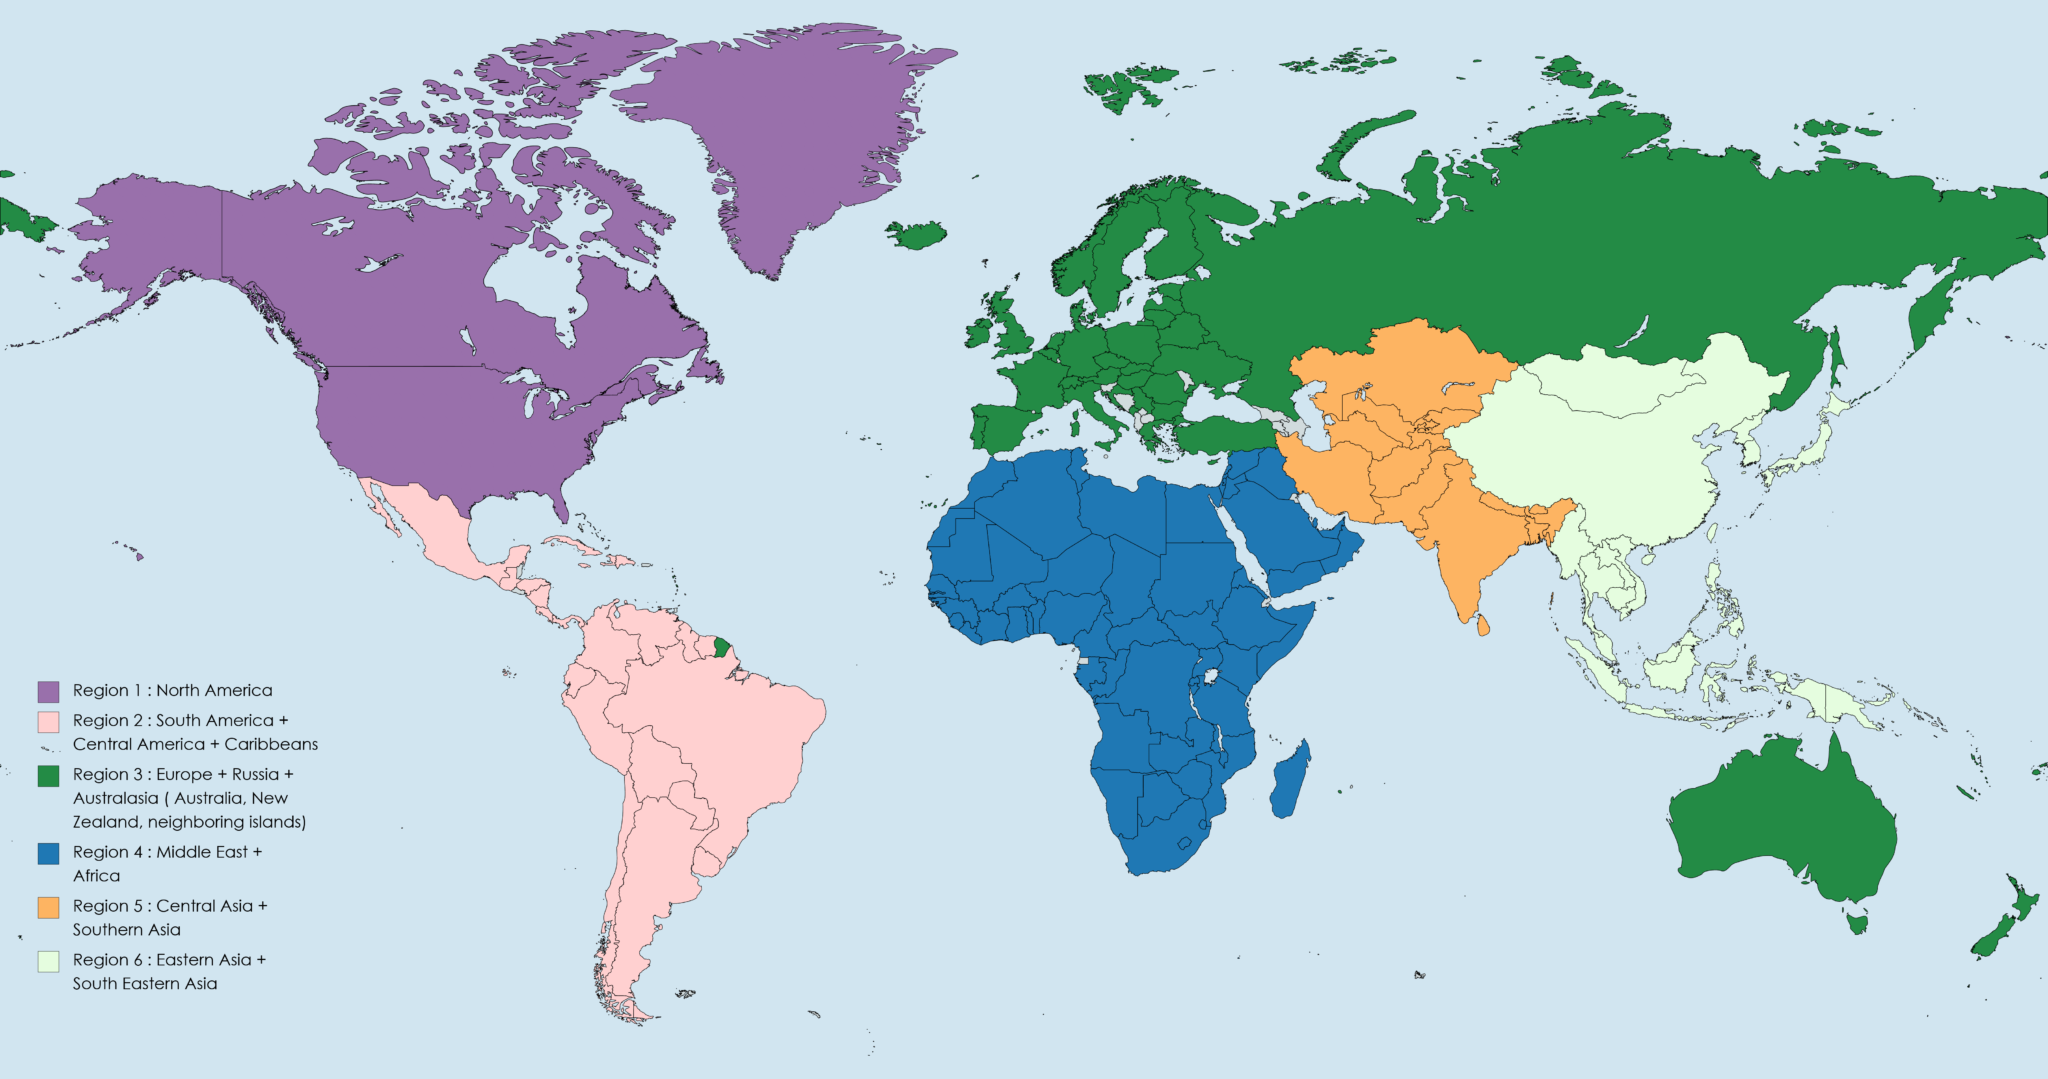
\includegraphics[width=\textwidth]{MapChart_Map-2048x1079.png}
    \caption{6 Different Regions}
\end{figure}

\begin{itemize}
    \item Region 1: North America
    \item Region 2: South America, Central America, Caribbeans
    \item Region 3: Europe + Russia + Australasia
    \item Region 4: Middle East + Africa
    \item Region 5: Central Asia + Southern Asia
    \item Region 6: Eastern Asia + South Eastern Asia
\end{itemize}

\subsection{Phases}

The competition was split into two phases.
In the first phase teams would submit their project ideas.
Then a number of teams per region are chosen as first phase winners.
Each winning team member is sent an OAK-D camera and the team as a whole gets access to Microsoft Azure and SuperAnnotate.
In the second phase it is up to the teams to realize their projects.

\subsection{OAK-D}

\href{https://store.opencv.ai/products/oak-d}{https://store.opencv.ai/products/oak-d} \\

The OAK-D is a 12MP 4k camera with two additional 1080P cameras on either side to provide depth information.
The camera housing also holds an Intel Myriad processor to run neural network inference on the camera footage directly on the device, without demanding the host PC.

\begin{figure}[H]
    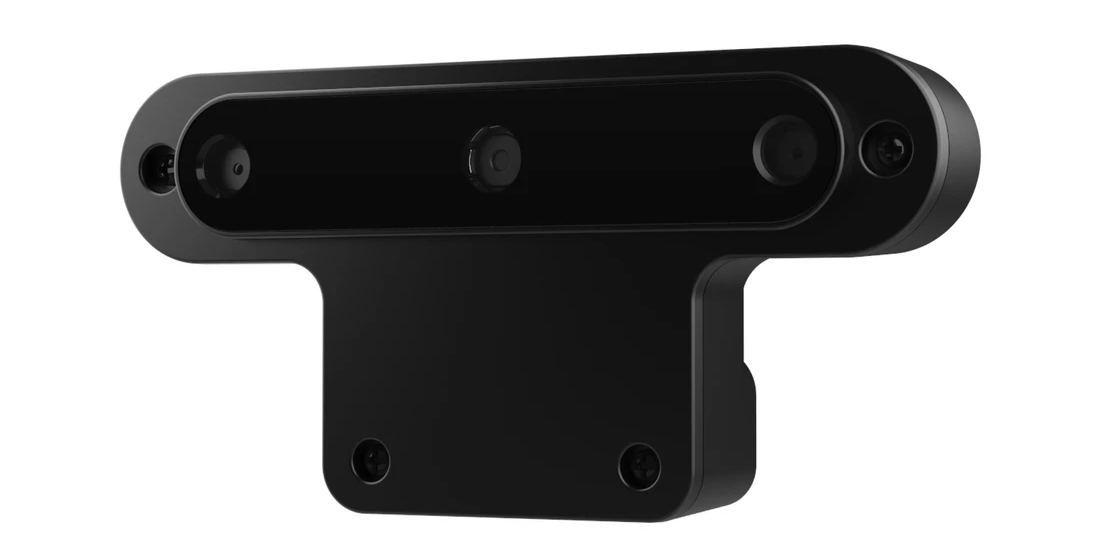
\includegraphics[width=\textwidth]{oakd-camera.png}
    \caption{OAK-D Camera}
\end{figure}

\begin{itemize}
    \item Integrated 4K 12 MP Color Camera
    \item JPEG, H.264 \& H.265/HEVC Encoding
    \item Integrated 1 MP Global Shutter Synchronized Stereo Pair
    \item USB 3.0 Type-C Interface
    \item Use with any host OS that OpenVINO supports
    \item Disparity-Depth Min Distance: 69cm
    \item Stereo AI (Stereo Inference Min Distance): 19.6cm
    \item Stereo Camera Hyperfocal Distance: 19.6cm
    \item Stereo Camera Baseline: 7.5cm
    \item Stereo Horizontal Field of View (HFOV): 71 degrees
    \item Stereo Camera Resolution: 1280×800
    \item RGB Camera resolution: 4056×3040
    \item RGB (AutoFocus) Min Distance: 8cm
\end{itemize}

\newpage
\section{The Team}

\subsection{Team Info}

\begin{tabular}{rl}
\textsc{Team Name:} & The German Mite Busters \\
\textsc{Categroy:} & Agriculture \\
\textsc{Region:} & Region 3 \\
\textsc & Europe + Russia + Australasia \\
\textsc & Germany \\
\textsc{Team Type:} & General Team \\
\end{tabular}

\subsection{Team Members}

\subsection*{Max-Felix Müller}
\begin{tabular}{rl}
\textsc{E-Mail:} & mxfxmmueller@gmail.com \\
\textsc{Credentials:} & Electrical Engineer - Embedded Software \\
\textsc & Pancake detector based on OpenCV \\
\textsc & Bottle classification using Jetson Nano \\
\textsc & Electric Wheelbarrow
\end{tabular}

\subsection*{Frank Münzner}
\begin{tabular}{rl}
\textsc{E-Mail:} & frank.muenzner@fpem.de \\
\textsc{Credentials:} & Electrical Engineer - Microsystems \\
\textsc & Premature failure analysis using OpenCV \\
\textsc & Object detection on Jetson Nano / Xavier \\
\textsc & Image detection and processing on LabView
\end{tabular}

\subsection*{Adam Müller}
\begin{tabular}{rl}
\textsc{E-Mail:} & adtheomueller@gmx.de \\
\textsc{Credentials:} & Mechatronics Engineer - Robotics \\
\textsc & 6-Axis Robot Arm \\
\textsc & Formula Student HHN - Head of Electronics
\end{tabular}

\subsection*{Lukas Dietz}
\begin{tabular}{rl}
\textsc{E-Mail:} & lukas.dietz@online.de \\
\textsc{Credentials:} & Software Engineer \\
\textsc & Formula Student Highspeed Karlsruhe - Head of Electronics \\
\textsc & X-Box CPU Modding
\end{tabular}

\newpage
\section{Submission}

The honey bee belongs to the class of insects, pollenising plants and therefore playing a significant role in nature not only in the survival of different types of plants but also as a basic requirement of our food supply.
In the last decade a considerable decline in honey bee population was observed.
There are many hypotheses about the possible causes.
Besides the use of insecticides, a major reason for bee mortality is the weakening of bee colonies by parasites.
The best known parasite is the varroa destructor.
It is assumed that up to 25\% of bee colonies in Germany do not survive the winter due to the infestation and the associated weakening by the mites. 

The varroa destructor is a parasitic mite, feeding on honey bees.
Furthermore, the mite carries bacteria and viruses into the bee colony.
The mite is about $ 2 mm^2 $ in size and attacks the bee by attaching to them and sucking the bees fat body.
The varroa mite lays eggs on the bee larva.
An infestation harms not only the bees directly affected, but may also lead to the death of the whole colony.

Currently there is no easy way to continuously monitor levels of varroa mites.
Some methods either harm or kill the bees, at least those used as a sample, or take a long time to get a result.
A possible method to get a continuous and timely overview of the size of the Varroa infestation would be to check the collecting bees flying in and out of the flyway for infestation.

Detecting the mites on the bees using computer vision will be a challenge due to the size alone.
Additionally the mites can attach to the bees not only from the top but also from the bottom, requiring multiple cameras to scan each bee.
We plan on mounting multiple cameras inside each bee hive, collecting as much data as possible.
The timing should be right, since the bees will very soon after the comeptition started also start flying again.

In a very first step, we focus on detecting the bees themselfs.
Counting the number of bees going in an out of the hive already gives insight on the health of the population.
When the classification is working, each bee can then be examined further, checking for pollen yield and the varroa destructor.

Most bee hives are further away from the city, making it difficult to stream images or videos to remote servers.
Using the OAK will enable us to run inference on location.
Only when a bee with the varroa destructor is detected, the owner of the hive will be notified.
He/She can also be notified if any irregularity in the behaviour of the bees is detected.

Reacting early is key in keeping our bees healthy and with the OAK and a suitable software, we can help the bees help us. \\

Thinking one step further, after the detection of the mites and notification of the owner we propose different mehtods of fighting the varroa destructor.

\begin{itemize}
    \item Selective killing of the mites by focused introduction of an active agent, dispatched using for example piezo electric dispensers.
    \item Local heating of the bee or prefferably the mite using a focused laser, either killing the mite directly or making it fall off the bee.
    \item Isolation and/or execution of the infested bee, which can then be trasported out by the worker bees.
\end{itemize}

\newpage
\section{Outputs while Getting Started}

Even while still getting started with the OAK-D and DepthAI API, there was some useful output produced that will be named here as a short summary.

Installing the DepthAI python module on the Jetson Nano threw some errors.
Together with the Discord community it was possible to identify the problem: a lack of RAM when running the Jetson Nano in desktop mode.
Apparently this does not happen when running headless, because the desktop environment seems to use about 1 GB of RAM.
Even though the higher RAM version of the Jetson Nano was used, there seemd to be a limit.
The solution was to add a swap file on the disk, in this case 4 GB were used.
This solution was also posted in Discord to help out others that run into the same problem.

Using an existing example model for object detection, its ouput was adapted to only show persons with increased threshold.
For the position of the person in the frame, the distance was estimated.
There were no fancy formulas used to calculate the distance, it is just a relative measurement.
After removing the output frame, the code can run headless.
It uploads the number of persons detected, as well as the distance to the closest person in the frame.
This can be used as a sort of presence detection, for example for home automation.

\newpage
\section{Designing the Pipeline}

The provided tutorials for getting started with DepthAI 2 API made it simple to understand the workflow using the API.
The procedure follows two steps: designing a pipeline and executing it.
The pipeline can be visualized as a real pipeline where the image and meta data is flowing through, following its course through different processing blocks.

When designing a pipeline the API offers different blocks to be used.
For example the camera input or a neural network inferencing block.
The blocks have different inputs and outputs that have to be connected together, respecting the data type of each.
To interface between the camera and the host PC, XLinks are used.
Such a XLink can transport any kind of information in a FIFO (first in, first out) queueing style.

During runtime, the PC has to fetch the data of all XLinks and handle it, depening on the datatype.
Some processing steps have to be done using the PC, but most heavy image processing can be done by the Intel Myriad processor on board the OAK-D, so the requirements for the host hardware remain low.
Each XLink queue can be designed blocking or non-blocking, meaning either the execution will wait for the next input or output which is good for keeping synchronization between different steps or run as fast as possible.

\begin{figure}[H]
    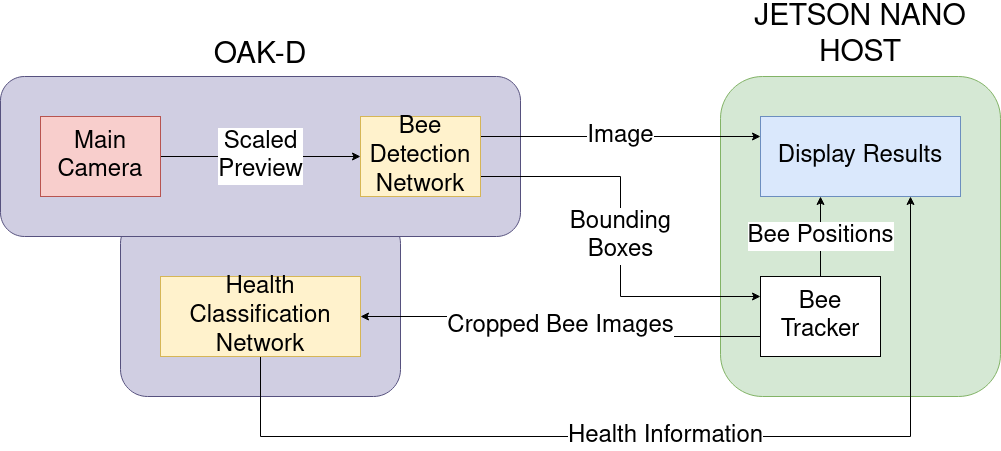
\includegraphics[width=\textwidth]{TGMB_Pipeline.png}
    \caption{Pipeline}
\end{figure}

The image above shows basic idea of the pipeline used for this project.
It tackles the task in two stages, first detecting the bees in the image and secondly checking their health.

The decision for a Jetson Nano as the host was made because it was laying around.
There are no specific requirements that would make one necessary.

\newpage
\subsection{Stage 1: Bee Detection}

To detect the bees, first an image has to be taken.
The image comes from the main camera of the OAK-D, a 12MP color camera.

Since the input size for the detection network is limited to a resolution of 300 x 300 pixels, the image has to be scaled down.
This can be done rather simple by requesting the preview image of the camera block to output a certain resolution and then passing on that instead of the main image.

The image can either be passed directly to the host, or with a passthrough through the network block.
The latter option has the advantage, that the network output will be in sync with the input image.
Otherwise smart handling of the incoming frame has to take place on the host side.

The detection network used outputs bounding boxes and labels.
The bounding boxes are the top left and bottom right coordinates of a rectangular box around the object.
The label holds the information what is detected inside the box.
In this project only bees are of interest and thus, there is only one possible class to be detected.

\subsection{Stage 2: Health Classification}

For each detected bee, the health has to be checked.
This can be easily done by a classification network, trained on healthy and infested bees.

This classification has to take place for every bee that was previously detected in the image.
At this point in time it is not yet possible to do that on the camera itself.
Instead, the frame with the detected bees has to be sent to the host PC.
There each bounding box can be cropped, resized to fit the classification network and then sent off to the OAK-D once more.

The classification will output the probability for each health status.
This information has to be received by the host and then decided on the most significant class.
For example 40\% healthy and 60\% varroa would be classified as infested.
The information has to be appended to the bounding box it belongs to and then displayed.

To have the input and output of this step synchronized, a blockin queue is used.

\newpage
\subsection{Pipeline in Python}

First the pipeline is defined as such.

\begin{lstlisting}
pipeline = dai.Pipeline()
\end{lstlisting}

The main camera is selected as the image source.
Its preview size is set as 300 x 300 to fit the input resolution of the neural network.

\begin{lstlisting}
cam_rgb = pipeline.createColorCamera()
cam_rgb.setPreviewSize(300, 300)
cam_rgb.setInterleaved(False)
cam_rgb.setFps(40)
\end{lstlisting}

Then the neural network is defined.
Its input is linked to the output of the camera preview.
Setting a threshold for the detection will remove guesses from the output, reducing further processing needs and eliminating false detections.
The number of inference threads allows the network to speed up.

\begin{lstlisting}
detection_nn = pipeline.createMobileNetDetectionNetwork()
detection_nn.setConfidenceThreshold(0.5)
detection_nn.setBlobPath(args.mobilenet_path)
detection_nn.setNumInferenceThreads(2)
detection_nn.input.setBlocking(False)
cam_rgb.preview.link(detection_nn.input)
\end{lstlisting}

The output of the network is sent to the host via a XLink.
Also the image of the camer is sent this way.
To keep them apart, each XLink has its own stream name.

Note that the image is first passed through the detection network and only then sent to the host, and not directly passed on from the preview output.
This will make sure that the network output is in sync with the frame it is derived from.

\begin{lstlisting}
xout_rgb = pipeline.createXLinkOut()
xout_rgb.setStreamName("rgb")
detection_nn.passthrough.link(xout_rgb.input)

xout_nn = pipeline.createXLinkOut()
xout_nn.setStreamName("nn")
detection_nn.out.link(xout_nn.input)
\end{lstlisting}

\newpage
For the second stage, the health classification, another network is created in the pipeline.
Since this network is way smaller, there is no need to configure much.
Also there is no threshold, because for each input (bee) an output is required.
This piece of the pipeline is also blocking, meaning execution will halt until a result is delivered.
This is important to make the connection between detected bee and health information.

\begin{lstlisting}
varroa_nn = pipeline.createNeuralNetwork()
varroa_nn.setBlobPath(args.varroa_path)
\end{lstlisting}

Since the classification network does not directly run on the captured image, its input instead comes from a XLink block.
For the second stage network, an input and output link are created with only the network in between.

Note that there is no direct connection between the bee detection stage and the health classification stage.
This connection has to be made by the host PC software.
In the pipeline image the "Bee Tracker" closes this gap.

\begin{lstlisting}
varroa_nn_xin = pipeline.createXLinkIn()
varroa_nn_xin.setStreamName("varroa_in")
varroa_nn_xin.out.link(varroa_nn.input)

varroa_nn_xout = pipeline.createXLinkOut()
varroa_nn_xout.setStreamName("varroa_nn")
varroa_nn.out.link(varroa_nn_xout.input)
\end{lstlisting}

\newpage
\section{Neural Network Workflow}

The basic workflow with neural networks is as follows:

\begin{enumerate}
    \item Define what the network should do
    \item Find or create a labeled dataset
    \item Find an existing network or build a new one
    \item Train the network (via transfer learning or from scratch)
    \item Convert to a blob file (specific to OAK devices)
    \item Run inferencing
\end{enumerate} 

This project will include all the tasks and even the different possibilities.
For example there is one dataset with labels included and one unlabeled.

\newpage
\section{Datasets}

Ideally for this project would be having access to a bee hive.
Contacting beekeepers proved more difficult than it should be, so for the beginning online datasets have to suffice.

While creating a dataset for bee detection would be simple enough, just place the camera in front of a hive, getting health information would be difficult.
Especially health information on a bee level is hard to come by for a non-professional.
So to detect varroa, the project will have to purely rely on freely available datasets.

\subsection{Kaggle}

"Kaggle is the world's largest data science community with powerful tools and resources to help you achieve your data science goals."

Kaggle is the probably best known source for datasets for machine learning online at the moment.
At least when not looking for a specific dataset.

The search for bees resulted in many datasets, out of which two were useful for this project.

\subsection{Bee Detection Dataset}

\href{https://www.kaggle.com/jonathanbyrne/to-bee-or-not-to-bee}{https://www.kaggle.com/jonathanbyrne/to-bee-or-not-to-bee} \\

To bee or not to bee is the question the dataset is asking.
Where is the bee would be a better question, but that is no reason to stop.
A better reason would be the fact, that the images are labeled only with the center position of each bee, and not with bounding boxes.

Bounding boxes are the borders of the object, in this case of the bee, that the detection network will produce as output.
They will have to be created manually in the next step.

There is another small problem with the dataset, since it was captured at a single location.
Therefore the background does only change over the time of the day.
That is good for a detection that will take place at that exact point, but is not good for generalizing the detection network.

\subsection{Health Classification Dataset}

\href{https://www.kaggle.com/jenny18/honey-bee-annotated-images}{https://www.kaggle.com/jenny18/honey-bee-annotated-images} \\

This dataset holds different bee types, health information, whether the bee holds pollen and many more informations.
For this project, the focus on health is enough.
The dataset distinguishes further between small varroa and varroa, a distinction that is not of interest for now.

In respect to the project goals, the dataset was split in 5 differnt classes: healthy, with varroa, queen missing, hive being robbed and attacked by ants.
For a second test, the dataset was reduced further to only differentiate between healthy and has varroa.

\subsection{Building a Bee Detection Dataset}

A small script was prepared by customizing the rgb full resolution saver example from the API.

The changes include 1080P resolution instead of 4K to reduce the amount of data.
If the image is downscaled to 300x300 for training anyhow, it does not make sense to capture more data.
On the other hand, having to do the job only once and getting the highest resolution possible would probably reduce the amount of work in the future.

Next, the framerate of the camera was reduced to 10 frames per second to reduce unnecessary load.
The capture of the data shall run at least a few hours, so more then one frame each second seems too much again.
The framerate however can not be set below 10 frames per second, otherwise the pipeline collapes during runtime.
Instead only every 10th image is stored and the other ones are discarted on the host computer side.

To get unique file numbers, the year, month, day, hour, minute and second are used.
In the worst case, this will lead to two files with the same name (due to rounding).
This does not matter, since for this task, there does not have to be a guaranteed "sample rate".

\begin{lstlisting}
for enc_frame in q_jpeg.tryGetAll():
frame_counter += 1
if frame_counter == 10:
    frame_counter = 0
    name = time.strftime('%Y %m %d %H %M %S')
    with open(f"{PATH}{name}.jpeg", "wb") as f:
        f.write(bytearray(enc_frame.getData()))
\end{lstlisting}

This is the code section for discarting the images and adding the timestamp to the name.
To make the time formatting readable spaces were added between each option.
The source code is available on GitHub.

These images then have to be labeled by hand, or with a service like SuperAnnotate.

\newpage
\section{LabelImg and SuperAnnotate}

To label unlabeled images, the OpenCV AI Competition offers the first phase winners a 200\$ credit for SuperAnnotate.
SuperAnnotate is an online service, allowing to upload images or videos that are later split into images.
On those images differnt objects can be marked by hand.
With the then labeled images, SuperAnnotate allows the training of a detection network.
Using this network, further images can be pre-labeled by the network itself, reducing the time it takes to label new images, because they only have to be checked and not labeled manually.

Although it seems interesting and fast, it certainly cuts a lot of learning opportunities and later there will be a lack of knowledge possibly leading to unexaplainable errors.
Instead, as a side project almost, the behaviour of SuperAnnotate will be reproduced.

The standard tool to label images for training a detection network is to use labelImg.
A tool desinged for labeling images for the tensorflow API.

labelImg allows loading of an images (or multiple images in a directory).
Then bounding boxes can be drawn by hand and a label can be added to the box.
For each images the tool produces and stores a xml file containing image information and the location and label of the boxes.

\subsection{DIY-SuperAnnotate}

Recreating the behaviour of SuperAnnotate is not too difficult.
At first, everything has to be done by hand once, but when that is done, the toolchain can be refined, making retraining of a network just a few clicks.
The difficulty then is to label the images.

Having access to the OAK-D solves this problem.
Instead of getting an image from the camera, a XLink input can be used to load the next image in the directory.
Then the original network on the OAK can run inferencing and will produce a number of bounding boxes.

On the host side, the bounding boxes are received and put with the correct formatting in an xml file, just as labelImg would do it.
This file can later be reopened by labelImg and necessary corrections can be made.
With the pre-labeling done by the network, further images can be labeled quicker than the first few.

\begin{figure}[H]
    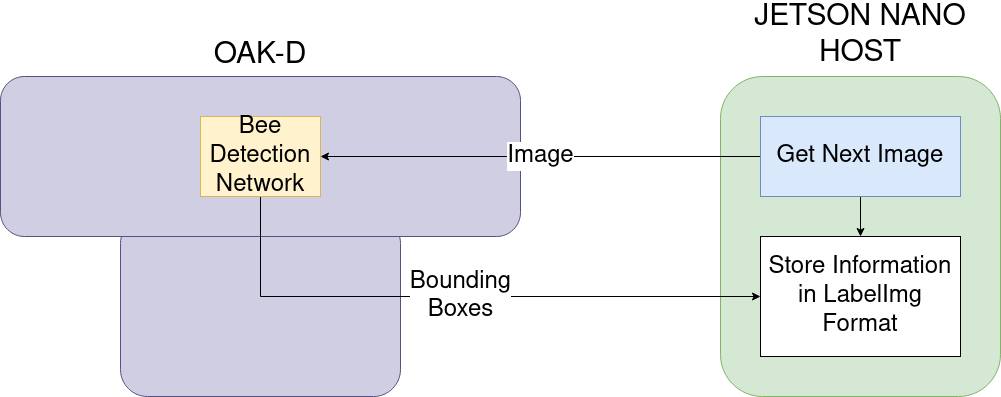
\includegraphics[width=\textwidth]{TGMB_SuperAnnotate.png}
    \caption{DIY SuperAnnotate}
\end{figure}

\newpage
\section{Bee Detection}

Winners of the first phase of the OpenCV AI Competition were supposed to get 200\$ for training networks on the Microsoft Azure cloud.
However the codes took a while to be distributed, so instead the project was mainly build and trained on Google Colab.

Google Colab is a Jupyter Notebook backend running on google servers and offers free access to GPUs and TPUs (Tensor Processing Units) for training.
There are also examples available for many different applications, such as training networks and converting them with the OpenVINO toolkit.

After finding a working example and fixing some problems with different versions, a working toolchain was done.
By adding new labels the training dataset can easily be increased and a new version of the model can be trained or the training of the old model can continue.

At first, it was not obvious that there is a difference between detection and classification networks.
After wondering a while how a classification network would output bounding boxes and reading some useful articles online, it was clear that there is a significant difference indeed.
Building a detection network from scratch requires massive amounts of data, so in this case, it is better to use an existing model and, if necessary, adapt it to the use case.

The model is a Mobilenet SSD (single shot detection) that is retrained to detect bees, which are not in the Coco dataset the network was previously trained for.
Transfer learning is used with the Tensorflow API, so that not the full network has to be retrained.
Different types of base networks were tested, with mixed results.

\subsection{OpenVINO and OpenVINO Version}

OpenVINO is a toolkit from Intel, used to convert models of different sources (Tensorflow, Caffe, PyTorch, ...) first to an intermediate representation (IR) and then to the blob file that can be loaded on the Myriad processor on the OAK-D.

The first example that was used was of version 2019-01.
It is not the newest one, but that was no problem at first.

When using two or more networks however, for example in a series pipeline like in this project, but also in a parallel pipeline, the OpenVINO version used to build the blob file must be the same.
This seems odd, because one would think, that the blob file is containing all information it needs to run, but apparently this is not the case.
During runtime there was an error requesting that the same OpenVINO version should be used for all models.
Since the OpenVINO version for the health classification network was 2021-01 it was easier to update the version here, then to downgrade the other one.

With the right installation commands, this was no challenge, but only a nuisance.

Searching the OpenVINO model zoo for models will also help find one that is possible to compile.
Training could be a waste of time, if it can not convert due to some reason later on.

\subsubsection{Shaves}

Another thing specific to the OAK-D and OpenVINO are shaves.
Shaves are Vector Processing Units (VPU) used for neural networks.
They can be thought of slices of the processor that can be used for different tasks.
There is a maximum of 16 shaves available on the OAK-D.
Depending on the camera resolution, either 10 when using 4K or 13 when using 1080P are available for neural networks (or other processing).
If no camera is used in the pipeline, the full number of shaves can be accessed by the blob file.

That means, when converting from the IR format to blob, the number of shaves must be chosen in a way that they "fit on the OAK-D".
Especially when using multiple networks in the pipeline, this has to be thought of beforehand.
Another option is obviously to compile the model for any number of shaves and later select which one to use.

\subsection{Mobilenet vs Resnet (and Yolo)}

Three pretrained networks were compared for the usage in the project.
Yolo v3, Mobilenet SSD v2 and ResNet 50 are the detection networks that were evaluated.

Yolo was not possible to train and compile with the toolchain build up in this project.

Mobilenet was, as the name implies, made to be run on mobile devices, meaning low power and low processing capabilities, at least when compared to workstations.
Smartphones are a possible target, for example to run image processing and applying beauty filters.
It has an average accuracy score in the comparison in the Tensorflow object detection model zoo.

ResNet on the other hand scores better, but is also slower.
In fact the number behind the name, 50 in this case, tells how deep the model is.
This model is about 50 layers too deep though, because when running inferencing on the OAK-D the framerate throttled to less then one frame per second.

Still, the outputs of the network had a subjectivly better accuracy then the ones from Mobilenet.
The performance drop was not 50\% as the comparison from Tensorflow would have made to believe.
Mobilenet runs with an average framerate of 25 frames per second.
Allowing more shaves when converting the IR format to the blob file with OpenVINO made no difference on the execution speed.

Another point for the ResNet was the larger input resolution of 640x640 compared to 300x300.
This is another reason why the network is slower.
There is a trick where the preview image is only used for the position of the bee in the frame, while the health classification would be run on a sub-frame of the full resolution one.
Changing the input resolution of a pre trained network is not possible, because for that the first layers would have to be adapted.
The whole reason why transfer learning works is because the first layers can be kept the same.
In that case, the whole network would have to be retrained, which is not possible for a small project with limited budget, because of the network size.

Due to the smaller network size, it was possible to train the Mobilenet model with a larger batch size.
The VRAM was limiting the batch size for the Mobilenet to 32 and for ResNet only 8.
To have a "fair" comparison, both networks were trained for 4 hours.

\subsection{Bee Detection in Google Colab}

The full code is available in the project GitHub.
Here are some highlighted code snippets and the reasoning behind them explained.

\subsubsection{While True Trick}

Colab is free to use, but it will disconnect after a certain time of inactivity.

When training a model, it might finish some time when nobody is there to continue or save the output (if not directly stored to a permanent storage).
To avoid this, simply build a while True loop, that will execute after the training.

\begin{lstlisting}
while True:
    pass
\end{lstlisting}

Anyways, the execution will disconnect from the GPU environment after 12h, so this is no "hack" that would enable free unlimited usage, just some convenience.

\subsubsection{Google Drive as Permanent Storage}

Since the runtime environment of Google Colab does not permanently keep any data, it makes sense to backup models, training checkpoints and datasets to Google Drive.
Especially when upload speed bandwidth is limited, this is a good option.
Of course, with the free account one is limited to 15GB, but that is plenty for small projects and afterwards, the important data can be downloaded and stored locally.

\begin{lstlisting}
from google.colab import drive
drive.mount("/content/gdrive")
\end{lstlisting}

\subsubsection{Access Files on Colab}

Gooogle offers modules to easily handle files in colab.

To make it clear to the user what to do next, a print statement was added in front.

\begin{lstlisting}
print("Upload my_resnet50.config now")
from google.colab import files
files.upload()
\end{lstlisting}

In this case, the configuration file supplied with the pre trained ResNet 50 model is outdated.
To allow the training to start sucessfully, the following two lines had to be added.

\begin{lstlisting}
fine_tune_checkpoint_type: "detections"
from_detection_checkpoint: true
\end{lstlisting}

This is to tell the training API, that the existing (pre trained) checkpoint is for a detection netwok.

With a similar construct it is possible to download files.
In this example, the compiled blob file.

\begin{lstlisting}
from google.colab import files
files.download(f"{ir_out_dir}/bee_detection.blob")
\end{lstlisting}

\subsubsection{Training in One Line}

Since the Tensorflow API is used to do the heavy lifting, training actually is just one single line of code.
The excalamation mark in front tells Colab that this has to be executed as a shell command, and not as a python command.

\begin{lstlisting}
!python -W ignore /object_detection/model_main.py \
    --pipeline_config_path={pipeline_fname} \
    --model_dir={model_dir} \
    --alsologtostderr \
    --num_train_steps={num_steps} \
    --num_eval_steps={num_eval_steps}
\end{lstlisting}

The directories and options were set beforehand and passed as variables to this command.

\newpage
\section{Health Classification}

The health classification network is build from scratch.
The base model is copied from an example, but it was extended by a few layers to make it deeper.
This can be critical, because too large of a network with too little data for training might result in overfitting.
Dropout should help reduce this though, and the training progress also does look promissing.

The network is a basic convolutional neural network with a couple fully connected layers at the end to get the scores for each class.

The currently used network was trained with about 2000 images for 100 epochs.
Each image is scaled 50x50, because they are samples of the 300x300 preview where the detection took place, so they can not be much larger.
The batch size was set to 32 for training.
The dataset was split 80\% for training and 20\% for validation.

Since most problems or problematic sections were already resolved while getting started with the first stage network, training a classification network proved to be easier.

\subsection{Health Classification in Google Colab}

The full code is available in the project GitHub.
Here are some highlighted code snippets and the reasoning behind them explained.

\subsubsection{Create Training and Validation Sets}

The dataset has to be split into training and validation.
The reasoning behind that is, that the network is not allowed to train with the same images that are later used to check its performance.
It would be like learning for an exam with the questions that will come.
Large (deep) networks might be able to overfit, meaning they "learn" the correct output for each image, but they will never be able to adapt to unseen or new inputs.

In this example the data is split 80\% for training and 20\% for validation.
Ideally there would be a third dataset for testing.

\begin{lstlisting}
train_ds = preprocessing.image_dataset_from_directory(
  data_dir,
  validation_split=0.2,
  subset="training",
  seed=123,
  image_size=(img_height, img_width),
  batch_size=batch_size)
\end{lstlisting}

The preprocessing is a function of Keras, a Python API for deep learning based on Tensorflow.

\subsubsection{The Model}

The model for the health classification was build from the ground up.
It is very close to the one from the example, except for some additional dense layers (so fully connected ones) at the end.

\begin{table}[H]
    \centering
    \begin{tabular}{||c c c||}
        \hline
        Layer (type) & Output Shape & Param \# \\
        \hline
        \hline
        sequential (Sequential) & (None, 50, 50, 3) & 0 \\
        \hline
        resizing (Resizing) & (None, 50, 50, 3) & 0 \\
        \hline
        rescaling\_1 (Rescaling) & (None, 50, 50, 3) & 0 \\
        \hline
        conv2d (Conv2D) & (None, 50, 50, 16) & 448 \\
        \hline
        max\_pooling2d (MaxPooling2D) & (None, 25, 25, 16) & 0 \\
        \hline
        conv2d\_1 (Conv2D) & (None, 25, 25, 32) & 4640 \\
        \hline
        max\_pooling2d\_1 (MaxPooling2) & (None, 12, 12, 32) & 0 \\
        \hline
        conv2d\_2 (Conv2D) & (None, 12, 12, 64) & 18496 \\
        \hline
        max\_pooling2d\_2 (MaxPooling2) & (None, 6, 6, 64) & 0 \\
        \hline
        dropout (Dropout) & (None, 6, 6, 64) & 0 \\
        \hline
        flatten (Flatten) & (None, 2304) & 0 \\
        \hline
        dense (Dense) & (None, 128) & 295040 \\
        \hline
        dense\_1 (Dense) & (None, 128) & 16512 \\
        \hline
        dense\_2 (Dense) & (None, 128) & 16512 \\
        \hline
        dense\_varroa (Dense) & (None, 5) & 645 \\
        \hline
    \end{tabular}
    \caption{Health Classification Model}
\end{table}

Total params: 352,293
Trainable params: 352,293
Non-trainable params: 0

The table is the summary of the model given by Keras.
Note that the last layer was given a specific name.
This was thought to be necessary to get the results when running inferencing on the OAK-D, but at the end it was not.

In the second column of the table, the output shape of each layer is given.
It is useful to have this information if a specific layer has to be extracted for debugging.

The last column shows the number of tunable parameters.
Meaning that many values have to be trained and later used to calculate the output, thus giving an idea of the size of the network.

Somewhere it was written, that for a good training one would need approximately 100 images (or input datas) per trainable parameter.
Just a quick look at this table makes it obvious that with about 2000 images for training this is no where near as good as it could be.

\subsubsection{Training}

Also with Keras, most of the work is done in the background.
To train the model, fit() is called.

There was an error in the original example notebook at this point, where the summary was looked at before training the model.
At that point the model does not "exist" yet, so it will throw an error.
To prevent this, first train the model and then look at the summary.
A small network like this also trains rather quickly, so having the summary available only after the training is not a problem.

As can be seen in the results, the accuracy improved really fast in the first few epochs, but then dropped.
However, due to the dropout layers added, the model kept improving, albeit slowly, during the whole training.

The curve is very close to 1 though, meaning there is the possibility of an overfit.
But the validation was also continuously improving, which would not happen if overfitting occured.

\begin{lstlisting}
epochs = 200

history = model.fit(
  train_ds,
  validation_data=val_ds,
  epochs=epochs
)

model.summary()
\end{lstlisting}

\begin{figure}[H]
    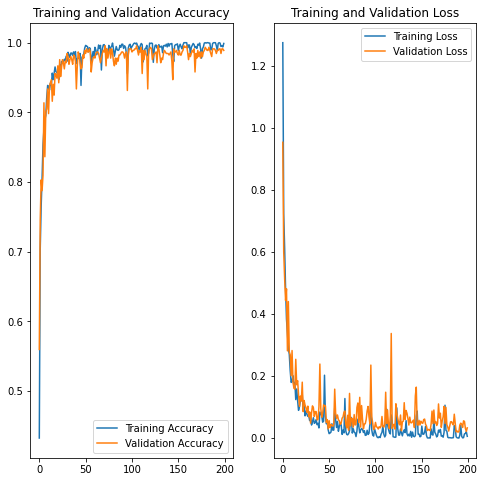
\includegraphics[width=\textwidth]{training.png}
    \caption{Training the Health Classification Network}
\end{figure}

Once the training completes, all that is left is compiling the model to a blob file and downloading it.

\newpage
\section{Building the Pipeline}

With the networks trained and exported as blob files and the outline of the pipeline in mind, it can now all be put together.
Once more the full code is available in the project GitHub.
Here are some highlighted code snippets and the reasoning behind them explained.

\subsection{Passing Detected Bees to the Classification}

In this part, the rectangle inside the detected bounding boxes is cut out and passed to the health classification network.

To achieve this, first the incoming detections are iterated one by one.
For each detection, the bounding box is scaled to the image (frame) size.

A bounding box position is defined by a number between 0 and 1 which represents the percentage.
In order to scale the positions, they have to be multiplied by the frame size in widht and height.

Since the frame is a numpy array at this point, "cutting out" the rectangle is only a matter of indexing.

The NNData object is used to transfer data across the XLink into the OAK-D.
In this case, the rectangle from the detection will have to be scaled to fit the network input layer (50x50) and flattened to fit into the data package.
The NNData object can then be sent.

\begin{lstlisting}
for det in detections:
    bbox = frame_norm(frame,
        (det.xmin, det.ymin, det.xmax, det.ymax))
    det_frame = frame[bbox[1]:bbox[3], bbox[0]:bbox[2]]
    var_data = dai.NNData()
    var_data.setLayer("0",
        to_planar(det_frame, (50, 50)))
    q_var_in.send(var_data)
\end{lstlisting}

\subsection{Receiving the Classification Result}

Receiving the results works by a blocking get call on the input queue.
This call has to be blocking to assure that the classification result goes with the current bounding box.
So before waiting for the queue it is possible to do some other quick lines of code (not visible here), since transmission to and from the OAK-D and inferencing will take a while.

\begin{lstlisting}
in_var = q_var_out.get()
result = np.array(in_var.getFirstLayerFp16())
result = health[np.argmax(result)]
\end{lstlisting}

Contrary to common sense the result is read from the first layer.
The reason is that when compiling the models to the IR format using OpenVINO an option is used to reverse the layers.

The classification returns an array with a percentage score for each possible class.
Using the argmax function finds the index with the highest score.
This index can then be used to select the label to print.

\subsection{Creating a Demo Video}

To create a demonstration of the network, output frames with marked labels and health informations are stored in a video file.
OpenCV has functions to create such a file.
The challenge in this case is, that the length of the video is unknown, the user might exit at any time.

Therefore, in a first step all the parameters have to be set.
The frame size is determined by the selected network and is stored in a dictionary that connects filenames to settings.

\begin{lstlisting}
fourcc = cv2.VideoWriter_fourcc(*'mp4v')
fps = 25 # this is assumed fps
size = networks[test_network]['size']
video = cv2.VideoWriter("video.avi",
    fourcc,
    fps,
    (size,size))

for frame:
    video.write(frame)

video.release()
\end{lstlisting}

The framerate of this video is locked.
However, the framerate of the pipeline is not fixed, because depending on the number of detections, the health classification will take longer.
The result is that in high framerate situations, the output video will appear slower than real-time, while during low framerates, it appears speed up.
An fps counter shows the correct framerate at any point in time, so the performance can be estimated even with the video.

\subsection{Bee Tracking in Python}

For being able to count the number of bees, be they healthy or infected, it is important to follow them through the frame.
Otherwise a single bee will get counted for each frame.

In this case a simple approach to tracking was chosen.
The center of each bounding box is defined as the bees position.
In the next frame, if a new position is very close to an old one, the bee is assumed to be the same.
This will not work cleanly when many bees are in the frame close together or even overlapping.

If a bee is not detected for an extended period of time, then its entry is cleared from the list of possible positions.
This can be the case if a false detection happens, or when the bee has left the frame.

An index is increased every time a bee enters the frame, so no id is used more then once.

Depending on the direction of the bee and at which side the frame was left, a counter can be implemented counting bees in the hive and the overall traffic.

\newpage
\subsection{Bee Tracking with the DepthAI Tracker}

The Python API for DepthAI comprises an object tracker.
It can be used on the output of a detection network and is able to track different objects, distinguished by their label, in one single block of the pipeline.
For tracking, the object tracker uses a kalman filter and the hungarian algorithm.
The kalman filter is used to estimate unkown system parameters, in this case for example the direction and the velocity of the tracked bee.
This estimation helps to make a minimal error while tracking.
The hungarian algorithm is used to make unique 1:1 connections between two groups, in this case for example the detections of the previous and the current frame.
When setting the tracker up, there are different mehtods of indexing and different tracking algorithms.

Since the health classification is added on top of the index, an index can not repeat.
Hence the unique ID is used for each tracked object.
This also means that if the tracker loses track of a bee, a new ID will be assigned to it and the health classification starts over.

The tracker requires three inputs: the detections, the frame the detections were made on, as well as the frame the tracking will be made on.
In this example setup the tracking and detection frame are the same.

\begin{lstlisting}
beeTracker = pipeline.createObjectTracker()

beeTracker.setDetectionLabelsToTrack([1])
beeTracker.setTrackerType(
    dai.TrackerType.ZERO_TERM_COLOR_HISTOGRAM)
beeTracker.setTrackerIdAssigmentPolicy(
    dai.TrackerIdAssigmentPolicy.UNIQUE_ID)

detection_nn.passthrough.link(
    beeTracker.inputDetectionFrame)
detection_nn.passthrough.link(
    beeTracker.inputTrackerFrame)
detection_nn.out.link(beeTracker.inputDetections)
\end{lstlisting}

\newpage
\section{Destruction}

When an infested bee is detected and classified as such, an immediate action is necessary.
The simple steps are notifying the owner that his bee(s) do carry the varroa destructor.
But to take it a step further, the infested bee would have to be separated and the mite has to be eliminated.

There are some proposed ways of handling with this.
For the project it was decided to go with the option to kill the mite with a focused laser beam.
As a proof of concept, a laser gimbal system was designed, that can be controlled via SALT, the System for Advanced Laser Targeting.

SALT consists of the hard- and software to track and destroy moving objects.

\subsection{Laser Gimbal}

For the first iteration of the laser gimbal hobby grade servos for RC cars were used.
Not the most expensive one as observed later.

Using a CAD program, in particular the online service OnShape, a few connecting parts were designed to fit the components together.
There are some design details to focus on.

The connecting parts have a hole in the middle for mounting the servo horns on the servos.
The connection is made with a screw and this holes allow the screw driver to reach through.

The connector between the first and the second servo is designed in a way that the laser diode is exactly centered on the first axis.
This is important to have the rotation of the laser along this axis in a predictable way.
If the laser were offset from the axis, the angle would be more difficult to compute later on.

\begin{figure}[h!]
    \centering
    \begin{subfigure}[b]{0.4\linewidth}
        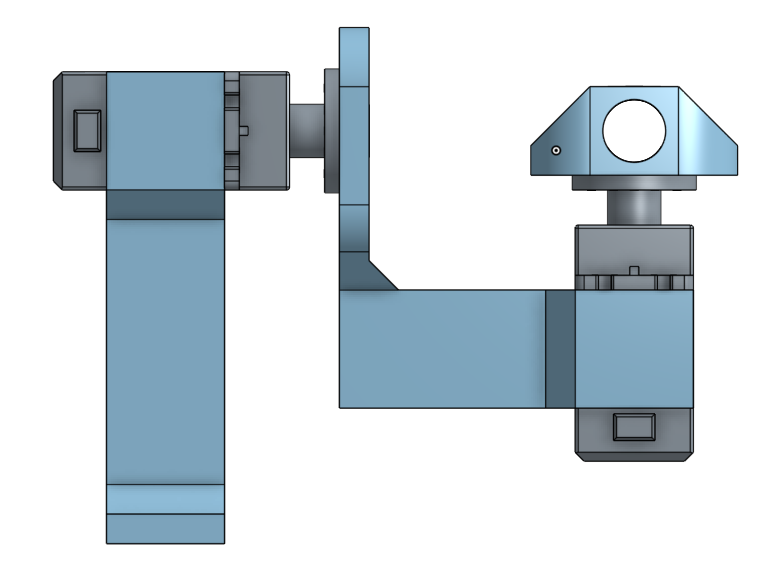
\includegraphics[width=\linewidth]{gimbal_front.png}
        \caption{Front View}
    \end{subfigure}
    \begin{subfigure}[b]{0.4\linewidth}
        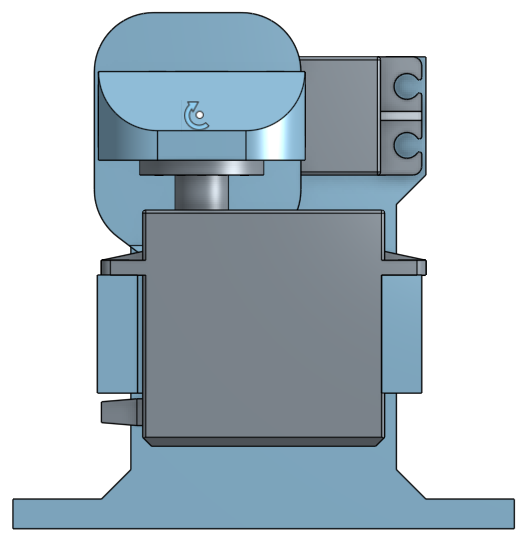
\includegraphics[width=\linewidth]{gimbal_side.png}
        \caption{Side View}
    \end{subfigure}
    \caption{Laser Diode Centered on both Axis}
\end{figure}

\newpage
\subsection{SALT}
Assume a flat surface, because hive entry is flat

SALT is the System for Advanced Laser Targeting.
It consists of the previously described laser gimbal, a controller for the servos and the software controlling it.

To control the servos a Teensy 4.1 was used generating the pulse width modulated signal.
It receives control commands over USB serial.
For this purpose, a protocol was created to interface with the gimbal software.

Different commands allow control over the x- and y-axis.
Also the laser can be controlled manually.
There is the possibility for an automated laser control mode.
In the automated mode the laser will switch on for a short time after reaching the requested position.

In addition to that a demonstration mode was programmed.
The demonstration mode has to be included during compilation of the source code.
That is a safety precaution, because the demonstration mode will disable normal functionallity while it is active.
This can not happen during operation.

The full desctiption of the available commands is in the code documentation on GitHub in the README.md file.

\subsection{Implementing SALT}

Finally all the parts could be put together.

When the detection network detects a bee in the frame its position information is kept track of with the bee tracker.
If the bee then is classified as infested with the varroa destructor mite, the position is sent over to the laser gimbal system.
Once the laser has reached the position, it turns on for a short burst to kill off the mite on the bee.

In theory at least.
With the limited time this is not possible.
Instead, the laser gimbal works as a proof of concept.
The infested bee will still be tracked and targeted, but the power of the laser is limited to just indicate its position and not to kill anything.

There is the option to send a "-d" or "--demo" as a command line argument.
For demonstration purposes the position of the lowest index in the tracker will be visualized by the laser.

\newpage
\section{Testing}

Testing was divided into different sections.
After each step of the process, tests were done to ensure the development was going in the right direction.
The last test session inside and then outside with real bees are documented here.

\subsection{Testing on the Bench}
\subsection{Gathering Real World Data}

To validate the network for bee detection in the field, real data was necessary.
The local bee keepers from "Bienenverein Flehingen e.v." allowed access to their hives.

\begin{figure}[H]
    \includegraphics[width=\textwidth]{gathering_field_data.jpg}
    \caption{Capturing Images and Videos with local Bee Keepers}
\end{figure}

For a general test of the system it was important not to capture hours of data on one single spot and angle, but to have as much variation as possible.
More test data can always be created, but the generalization of the model can only be validated this way.
Too much of the same would only lead to difficulties in the analysis.

All in all, about 10 minutes of data was captured.
The script was modified to not only capture video data, but at the same time output each encoded frame.
Since the direct frames would be too similar, only one frame per second was saved as an image.
This way, about 600 images were captured.

The 600 images show different hives, with different openings, different lighting and different angles.

When capturing images of bees it is important to approach the hive from the back.
Then it is possible to observe the bees.
Standing in the direction that the bees are currently flying towards and coming back from is not advised.
Instead, choose an angle were the bees are currently not flying.
This is generally save and neither persons nor bees were harmed in the process.

\subsection{Testing in the Field}

\newpage
\section{Fixes and Improvements}

\subsection{Implemented Improvements}

The synchronization between the image and the neural network results was not given at first.
This lead to the detection box always appearing offset from the real bee in the image.
The fix was to use the passthrough in the pipeline of the neural networks.
Also in the code, it is better in this case to wait for all data to come in and only then showing the new frame on the screen.

Bee tracking was improved by switching from a very simple tracker in Python to the included object tracker from DepthAI.
There are further improvements possible, they are listed in the next section.

\subsection{Further Improvements}

\subsubsection{Improving the Dataset}

The labeling of bees was done manually.
Since there was no prior experience, every bee was labeled.
Even the ones where only part of the bee was visible, because other parts were obstructed, for example by the entry of the hive.
This lead to all round, dark things being detected as bees.
A possible improvement would be relabeling only the completely visible bees in all the images and retraining the networks.

The training dataset only holds data from one location.
Every picture has the same background, making it relatively easy for the network to learn, but at the same time harder to generalize.
During the project images were collected from two different locations, different hives and from different angles.
Once these images are labeled they can be used for training as well.
This will greatly improve generalization.

Furthermore, the newly collected data also includes bees at different distances from the camera.
The original training dataset used a camera with a fixed distance to the hive entry, again making it more difficult for the network to generalize.

To improve on the health classification it could be beneficial to use higher resolution inputs.
This can be achieved by not cropping the 300x300 output image of the bee detection network, but using the detected bee positions and cropping the bee from the original high resolution frame.
The position is already given in relative coordinates, so it would be easy to map them on the original frame.

\subsubsection{Improving the Tracking System}

The tracking system could be further improved by using the depth information.
With a 3D trajectory estimation, the bees can be tracked more accuratly, especially during flight.
Additionally, this would provide depth information that can be used for the next idea.

\subsubsection{Improving the Laser System}

The laser (if it is not perfect) could be focussed on the mite exactly by using the depth information from the OAK-D.

To improve the speed of the laser system, a laser galvanometer should be used.
Instead of moving the laserdiode to aim, the galvanometer uses small mirrors to steer the beam.
This is faster, because the mirrors are lighter and thus they can be moved more quickly.

\subsection{Lessons Learned from an Expert Interview}

The time with the "Bienenverein Flehingen e.v." was used to interview bee keepers about their experience with the varroa destructor.

The varroa destructor is in every hive.
There are no bee populations without at least some mites.
This is not too bad, as long as the total number of mites stays within some limit.

According to the experts, the mite itself does not have a reason to fly with the worker bees out of the hive.
Most of them are inside the honeycombs where the larva life.
Therefore it is not clear, if the number of mites counted on the worker bees going in and out of the hive is proportional to the count inside the hive.

Currently the best option for estimating the varroa destructor infestation is to clean out the dirt that collects in the bottom of the hive and count the number of mites in there.
This is a highly manual work, because the mites have to be separated from the dust to count them.
A possible solution to ease the job for the bee keepers would be to have a camera system that can count the number of mites inside this dirt from a single picture.

Using a laser system to kill the varroa destructor was not favored by the bee keepers.
The heat of the laser would not only heat up the mite, but also the bee.
According to their knowledge, the mite would indeed die first, but the difference in temperature needed to kill the mite versus the temperature that puts the bee in danger is too small.
It is not worth to take that risk.

A good enough solution would be to simply count the number of varroa mites going in and out of the hive and then estimating the number of mites inside.
As stated, there is nearly no bee population with no mites anymore, making a simple detection useless.
Instead a large increase in the count could be evidence to move the population to a new hive and keep the bee population alive.

\newpage
\section{Special Thanks}

We want to thank the beekeepers of the Bienenverein Flehingen e.v. for allowing us access to their bees.
It was a unique opportunity to have real world data and some thoughts of experts on the field.\\

We also want to thank the organizers of the competition for enabling this project and for giving us the opportunity to experiment with DepthAI, the OAK-D and SuperAnnotate.

\newpage
\section{Links}

Links to ressources and project files: \\

OpenCV AI Competition 2021

\href{https://opencv.org/opencv-ai-competition-2021/}{https://opencv.org/opencv-ai-competition-2021/} \\

OAK-D Camera

\href{https://store.opencv.ai/products/oak-d}{https://store.opencv.ai/products/oak-d} \\

TGMB on GitHub

\href{https://github.com/MxFxM/TGMB}{https://github.com/MxFxM/TGMB} \\

Bee Detection Dataset on Kaggle

\href{https://www.kaggle.com/jonathanbyrne/to-bee-or-not-to-bee}{https://www.kaggle.com/jonathanbyrne/to-bee-or-not-to-bee} \\

Bee Health Classification Dataset on Kaggle

\href{https://www.kaggle.com/jenny18/honey-bee-annotated-images}{https://www.kaggle.com/jenny18/honey-bee-annotated-images} \\

LabelImg

\href{https://github.com/tzutalin/labelImg}{https://github.com/tzutalin/labelImg} \\

OpenVINO Model Zoo

\href{https://github.com/openvinotoolkit/open_model_zoo}{https://github.com/openvinotoolkit/open\_model\_zoo} \\

\end{document}
